\documentclass{beamer}
\usetheme{Boadilla}
\usepackage{essay-def}
\usepackage{bm}
\usepackage{amsfonts}
\usepackage{amssymb}
\usepackage{amsmath}
\usepackage{amsthm}
\usepackage{comment}
\usepackage{geometry}
\geometry{left=1cm,right=1cm}
    \title[Comp \& Stat OT]{Computational and statistical optimal transport}
\author[J. Zhao]{Jiaxi Zhao}
%\institute[]{joint work with Wuchen Li (UCLA)}
\date{26th May, 2021}
\begin{document}
\par \setlength{\parindent}{2em}

\begin{frame}
\titlepage

\end{frame}


\begin{frame}{Brief history of optimal transport}
    \begin{figure}[H]
          \centering
          \centerline{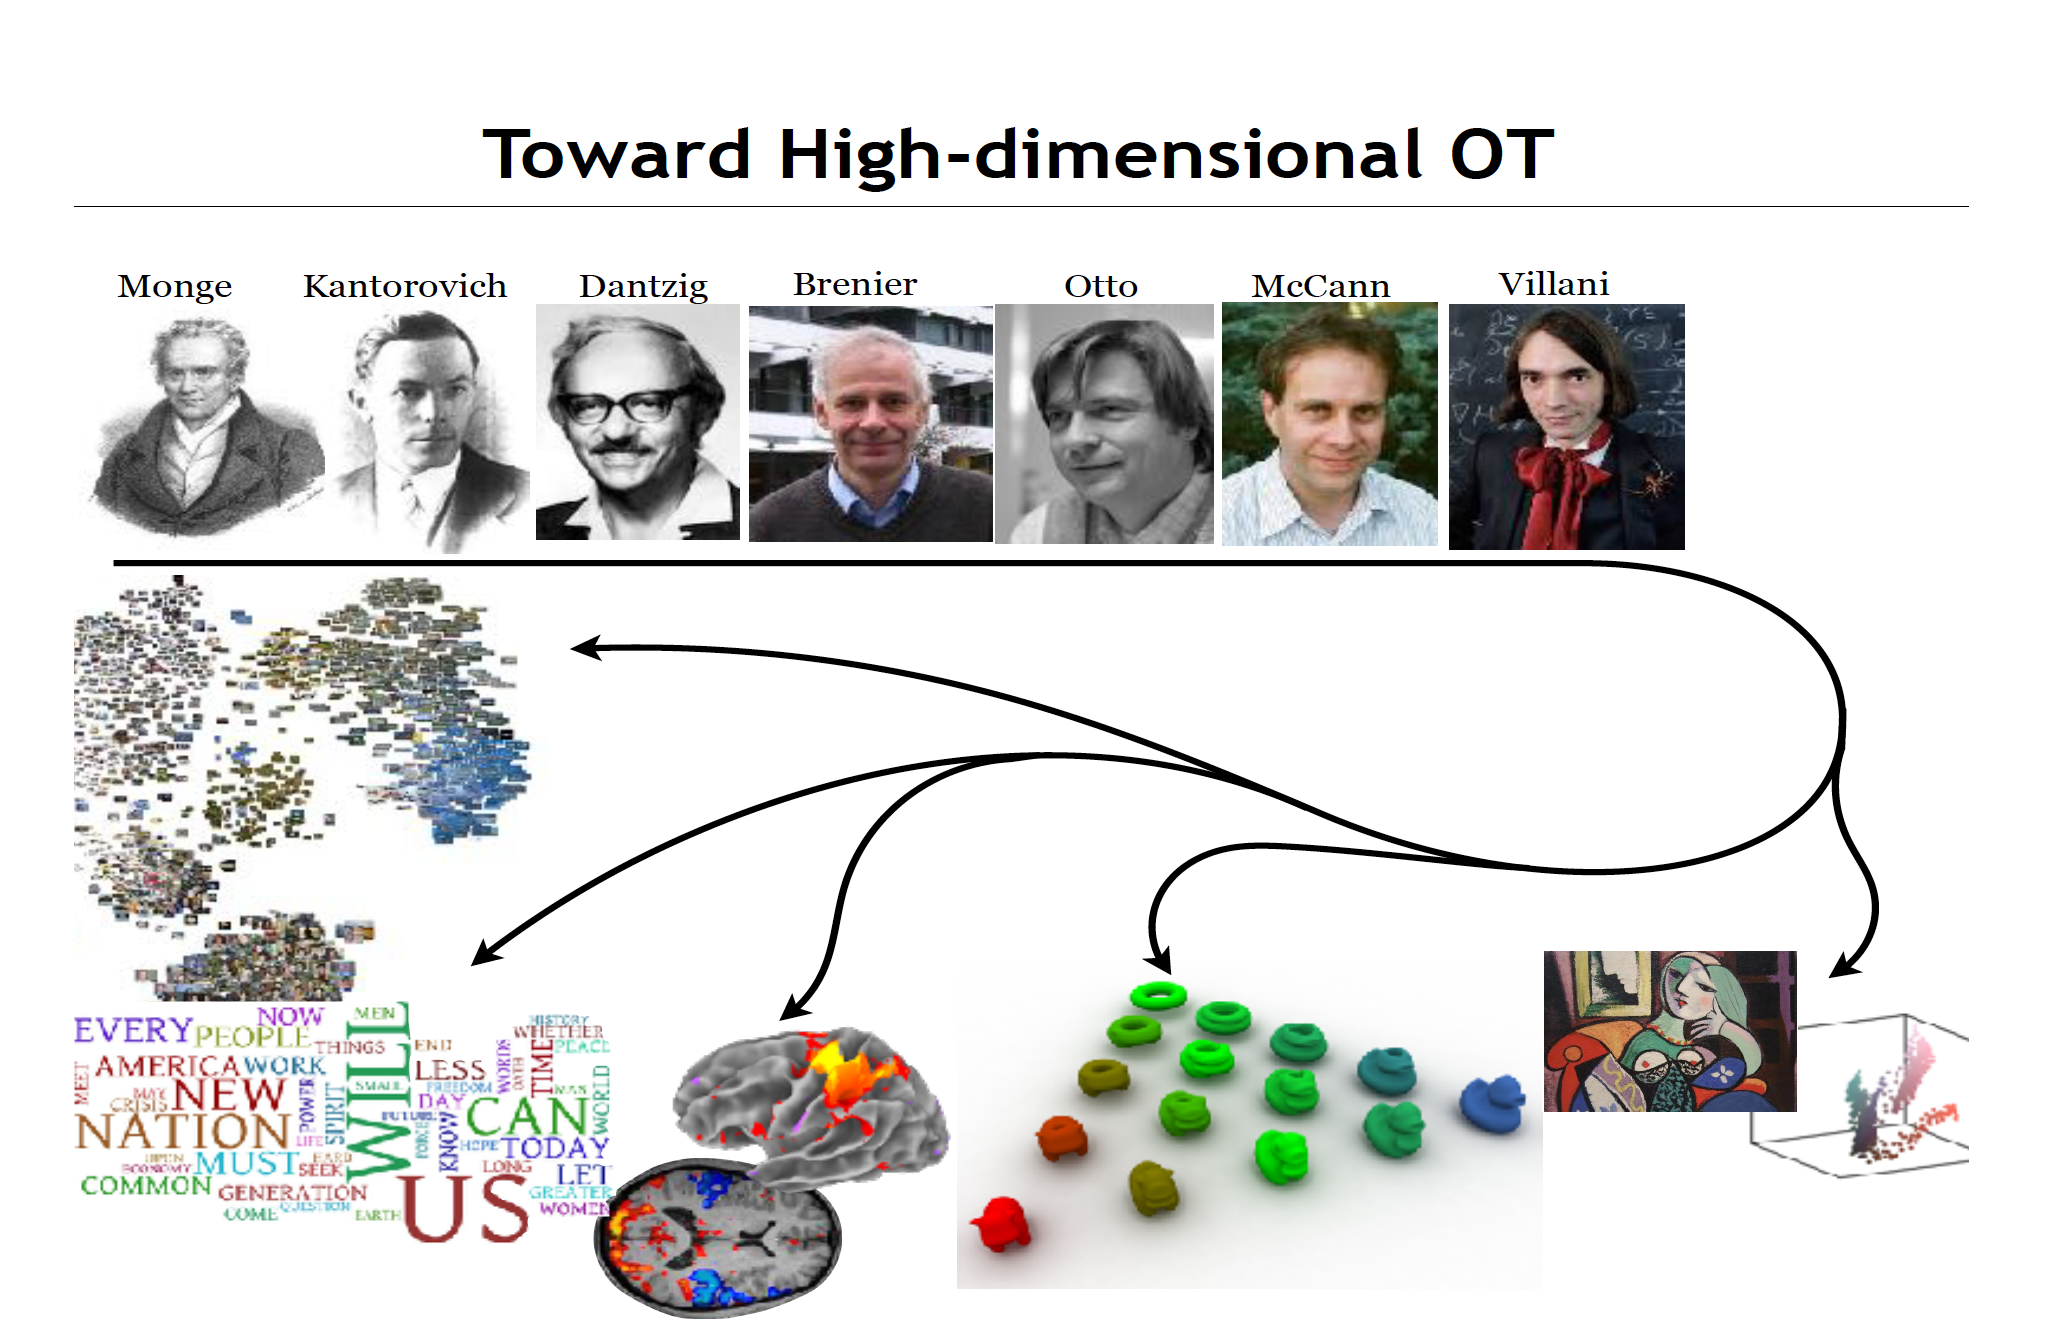
\includegraphics[width=\linewidth]{history.png}}
          \caption{Copied from Prof. S. Justin's lecture note.}
        \end{figure}
\end{frame}


\begin{frame}{Optimal transport: Monge formulation}
	Given two target distribution $\mu, \nu$ in space $X, Y$ and a cost function $c(\cdot, \cdot): X \times Y \rightarrow \mbR_{\geq 0}$, we consider to find a mapping $f: X \rightarrow Y$ such that $f_*\mu = \nu$ and minimize the total cost 
	\bequn
		C = \int_{X} c(x, f(x)) \mu(x) dx.
	\eequn
	Usual types of cost:
	\begin{itemize}
		\item $L^p$ cost.
		\item 0-1 cost, total variation.
	\end{itemize}
	Related topics: Monge-Amp\`ere equation.
\end{frame}

\begin{frame}{Optimal transport: Kantorovich formulation}
Kantorovich provided a relaxed version of this problem, relax from deterministic coupling to stochastic coupling. 
\bequn
		\begin{aligned}
			W_c\lp \mu, \nu \rp & = \inf_{\pi \in \prod\lp \mu, \nu \rp} \int c\lp x, y \rp d\pi\lp x, y \rp,		\\
			W_p^p\lp \mu, \nu \rp & = \inf_{\pi \in \prod\lp \mu, \nu \rp} \int \lv x - y \rv^p d\pi\lp x, y \rp \ \text{(Wasserstein-p distance)}.
		\end{aligned}
	\eequn
Denote $X_0\sim \mu_0=\delta_{x_0}$, $X_1\sim \mu_1=\delta_{x_1}$. Compare
$$W(\mu_0,\mu_1)=\inf_{\pi\in\Pi(\mu_0, \mu_1)}\mathbb{E}_{(X_0, X_1)\sim\pi} c(X_0, X_1)=c(x_0,x_1);$$
Vs
$$\textrm{TV}(\mu_0,\mu_1)=\int_{\Omega}|\mu_0(x)-\mu_1(x)|dx=2;$$
Vs 
$$\textrm{KL}(\mu_0\|\mu_1)=\int_\Omega\mu_0(x)\log\frac{\mu_0(x)}{\mu_1(x)}dx=\infty.$$
\end{frame}


\begin{frame}{Linear programming formulation}
\par
	If we use histograms to replace the distributions in previous formula, i.e. $\mu \in \mbR^n, \mu \in \mbR^m$ with $\mathbf{1}^T\mu = \mathbf{1}^T\nu = 1$, we will obtain linear programming (matrix) formulation of the optimal transport, i.e.
	\bequ
		\begin{aligned}
			& \min_{\mfP \in \prod(\mu, \nu)}\la \mfC, \mfP \ra,			\\
			& \prod(\mu, \nu) := \left\{ \mfP \in \mbR^{n \times m} | \mu = \mfP\mathbf{1}, \mathbf{1}^T\mfP = \nu^T \right\},			\\
		\end{aligned},
	\eequ
	here $\mfC \in \mbR^{n \times m}$ is the elementwise cost function. \\
	A LP with $mn$ unknown variables and $m + n$ constraints, which is extremely hard to calculate when $m, n$ is large.
\end{frame}


\begin{frame}{Classifications of computational OT}
\par
There exist several different classifications of OT:
\par
\textbf{1. Classification by the target and source distribution:}
\begin{itemize}
	\item Discrete OT (LP)
	\item Semi-discrete OT (Voronoi diagram)
	\item Continuous OT
\end{itemize}
\par
\textbf{2. Classification by algorithms:}
\begin{itemize}
	\item Sinkhorn distance
	\item Semi-dual OT, only applied to Wasserstein-2
	\item Projected Wasserstein distance
\end{itemize}
\par
\textbf{3. Different goal:}
\begin{itemize}
	\item Calculate distance
	\item Calculate mapping, vector field
\end{itemize}
\end{frame}


\begin{frame}{Sinkhorn's algorithm and Sinkhorn divergence}
\par
One famous in the computational OT is the Sinkhorn algorithm. In the original paper\footnotemark, the Sinkhorn distance is defined as 
	\bequ
		d_{\alpha}\lp \mu, \nu \rp = \min_{\pi \in \prod_{\alpha}(\mu, \nu)}\lbb \int_{\mcX \times \mcY} c(x, y)d\pi(x, y) \rbb = \min_{\mfP \in \prod_{\alpha}(\mu, \nu)}\la \mfC, \mfP \ra,
	\eequ
	where the set $\prod_{\alpha}(\mu, \nu) := \lbb \pi \in \prod(\mu, \nu) | H(\pi | \mu \otimes \nu) \leq \alpha \rbb$ with $H(\cdot | \cdot)$ the relative entropy. Entropic OT appearing as the Lagrangian function of the Sinkhorn distance, i.e.
	\bequ
		\begin{aligned}
		W_{\epsilon}\lp \mu, \nu \rp = & \ \min_{\pi \in \prod(\mu, \nu)}\lbb \int_{\mcX \times \mcY} c(x, y)d\pi(x, y) + \epsilon H(\pi | \mu \otimes \nu) \rbb \\
		= & \ \min_{\mfP \in \prod(\mu, \nu)}\la \mfC, \mfP \ra - \epsilon H(\mfP).
		\end{aligned}
	\eequ
\footnotetext{M. Cuturi. Sinkhorn distances: Lightspeed computation of optimal transport. Advances in neural information processing systems, 26:2292–2300, 2013.}
\end{frame}


\begin{frame}{Sinkhorn's algorithm}

\begin{figure}[h]
	\centering
  	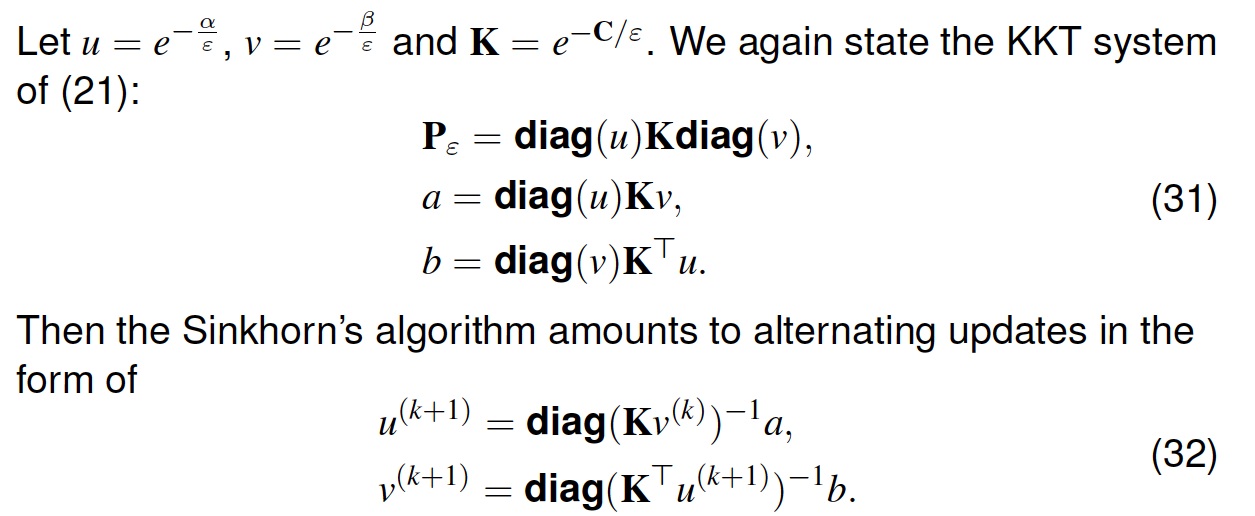
\includegraphics[width=\linewidth]{Sinkhorn.png}
  	\caption{Sinkhorn's algorithm}
  	\label{Sinkhorn}
\end{figure}
It is proved in\footnotemark that the Sinkhorn's algorithm converges in linear rate with an $\epsilon$ depending constant $e^{\frac{1}{\epsilon}}$. 
\footnotetext{C. Brauer, C. Clason, D. Lorenz, and B. Wirth. A sinkhorn-newton method for entropic optimal transport. arXiv preprint arXiv:1710.06635, 2017.}
\end{frame}


\begin{frame}{Properties of the Sinkhorn divergence}
	Approximation power of Sinkhorn divergence
	\begin{Thm}[A. Genevay et. al, 2019]
	Let $\mu, \nu$ be probability measures on $X, Y$ respectively, subsets of $\mbR^d$ such that $\lv X \rv, \lv Y \rv \leq D$ and
assume that $c(x, y)$ is $L$-Lipschitz w.r.t. $x, y$. It holds
		\bequ
			0 \leq W_{\epsilon}\lp \mu, \nu \rp - W\lp \mu, \nu \rp \leq 2\epsilon d\log \frac{e^2LD}{\epsilon\sqrt{d}} \sim 2\epsilon d\log \frac{1}{\epsilon}.
		\eequ
	\end{Thm}
	\bequn
		W_{\epsilon}\lp \mu, \nu \rp = \inf_{\rho, v}\int_0^1\int_{\Omega} \lp \norml v(x, t) \normr^2 + \frac{\epsilon^2}{4}\norml \nabla \log \rho(x, t) \normr^2 \rp dxdt.
	\eequn
	\bequ
		\lv \mbE_{\pi_{\epsilon}}\norml x - y \normr^2 - W_2^2(\mu, \nu) \rv \leq \left\{
		\begin{aligned}
			&O(\exp(-1/\epsilon)), \quad \text{discrete OT (LP)},		\\
			&O(\epsilon^2), \quad \text{semi-discrete OT},		\\
			&O(\epsilon), \quad \text{continuous OT}.		\\
		\end{aligned}\right.
	\eequ
\end{frame}


\begin{frame}{Properties of the Sinkhorn divergence}
	Sample Complexity of Sinkhorn divergence
	\begin{Thm}[A. Genevay et. al, 2019]
		Let $\mu, \nu$ be probability measures on $X, Y$ respectively, subsets of $\mbR^d$ such that $\lv X \rv, \lv Y \rv \leq D$ and
assume that $c(x, y)$ is $C^{\infty}$, $L$-Lipschitz w.r.t. $x, y$. One has
		\bequ
			\mbE\lv W_{\epsilon}\lp \mu, \nu \rp - W_{\epsilon}\lp \wht \mu_N, \wht \nu_N \rp \rv = O\lp \frac{e^{\frac{\kappa}{\epsilon}}}{\sqrt{n}}\lp 1 + \frac{1}{\epsilon^{\lfloor \frac{d}{2} \rfloor }}\rp \rp,
		\eequ
		with $\kappa = 2L\lv X \rv + \norml c \normr_{\infty}$.
	\end{Thm}
\end{frame}


\begin{frame}{Other regularization}
	Entropic OT has the following drawback that it breaks the sparsity in the intrinsic LP formulation. Can we use other regularization to obtain better approximate solution?
\end{frame}


\begin{frame}{CoD in OT computation}
	\begin{Thm}[Boissard et. al, 2014.]
		Let $\mu$ be a probability measure on $[-1, 1]^d$. If $\mu_n$ is an empirical measure comprising $n$ i.i.d. samples from $\mu$, then for any $p \in \lb 1, \infty \rp$,
		\bequ
			\begin{aligned}
				\mbE W_{p}(\mu, \mu_n) \leq r_{p, d}(n) := c_p\sqrt{d}\lbb\begin{aligned}
					& n^{-\frac{1}{2p}}, \quad d < 2p,	\\
					& n^{-\frac{1}{2p}}(\log n)^{\frac{1}{p}}, \quad d = 2p,		\\
					& n^{-\frac{1}{d}}, \quad d > 2p.
				\end{aligned}\right.
			\end{aligned}
		\eequ
	\end{Thm}
\end{frame}


\begin{frame}{More on OT}
	\begin{figure}[H]
          \centering
          \centerline{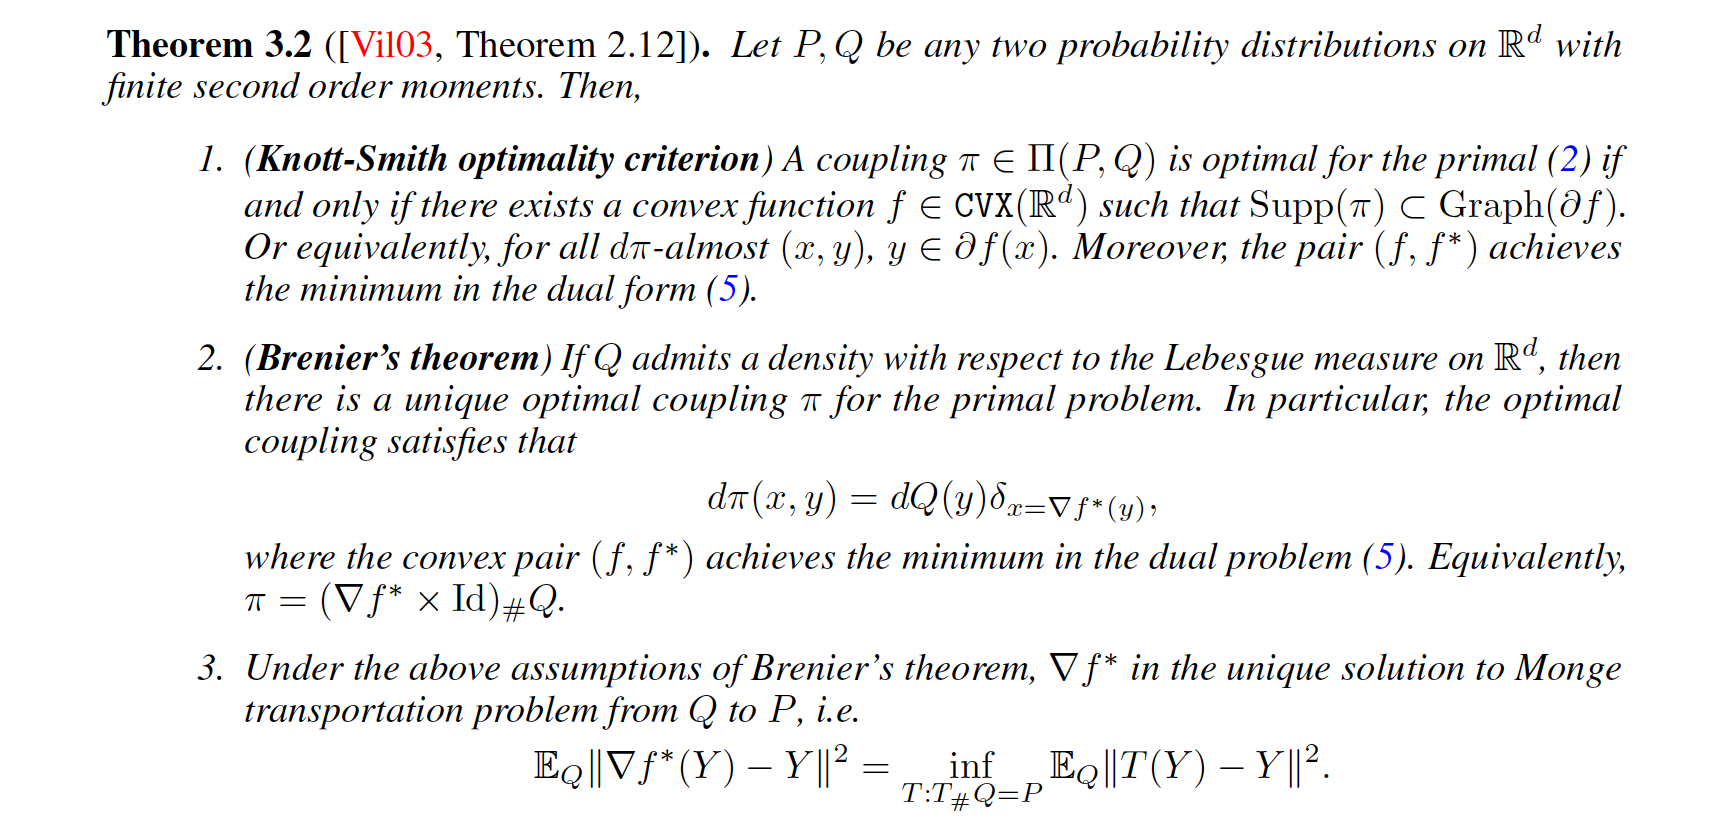
\includegraphics[width=1.2\linewidth]{Brenier.png}}
          \caption{Struture theorem for $L^2$ OT.}
        \end{figure}
\end{frame}


\begin{frame}{Semidual formulation}
	\bequn
		\begin{aligned}
			W_2(\mu, \nu) = & \min_{X,Y \sim \mu, \nu}\mbE \norml X - Y \normr_2^2		\\
			= & \ \min_{X,Y \sim \mu, \nu}\lp \mbE \norml X \normr_2^2 + \mbE \norml Y \normr_2^2 - 2\mbE \la X, Y \ra \rp 	\\
			= & \  \mbE \norml X \normr_2^2 + \mbE \norml Y \normr_2^2 - 2\max_{X,Y \sim \mu, \nu}\mbE \la X, Y \ra.
		\end{aligned}
	\eequn
	Use Lagrangian multiplier on this maximum term, we obtain for any two probability distributions $\mu$ and $\nu$ on $\mbR^d$ with finite second order moments, we have that
	\bequn
		\max_{X,Y \sim \mu, \nu}\mbE \la X, Y \ra = \inf_{f cvx} \mbE_{\mu}f(X) + \mbE_{\nu}f^*(Y),
	\eequn
	where $f^*$ is convex conjugate.
\end{frame}


\begin{frame}{Semidual formulation: semidiscrete OT}
	In semidiscrete case, the potential function has special form, it is the maximum of finite many linear function
	\bequn
		f(x) = \max_{i} (y_i^t x + b_i).
	\eequn
	\begin{figure}[H]
          \centering
          \centerline{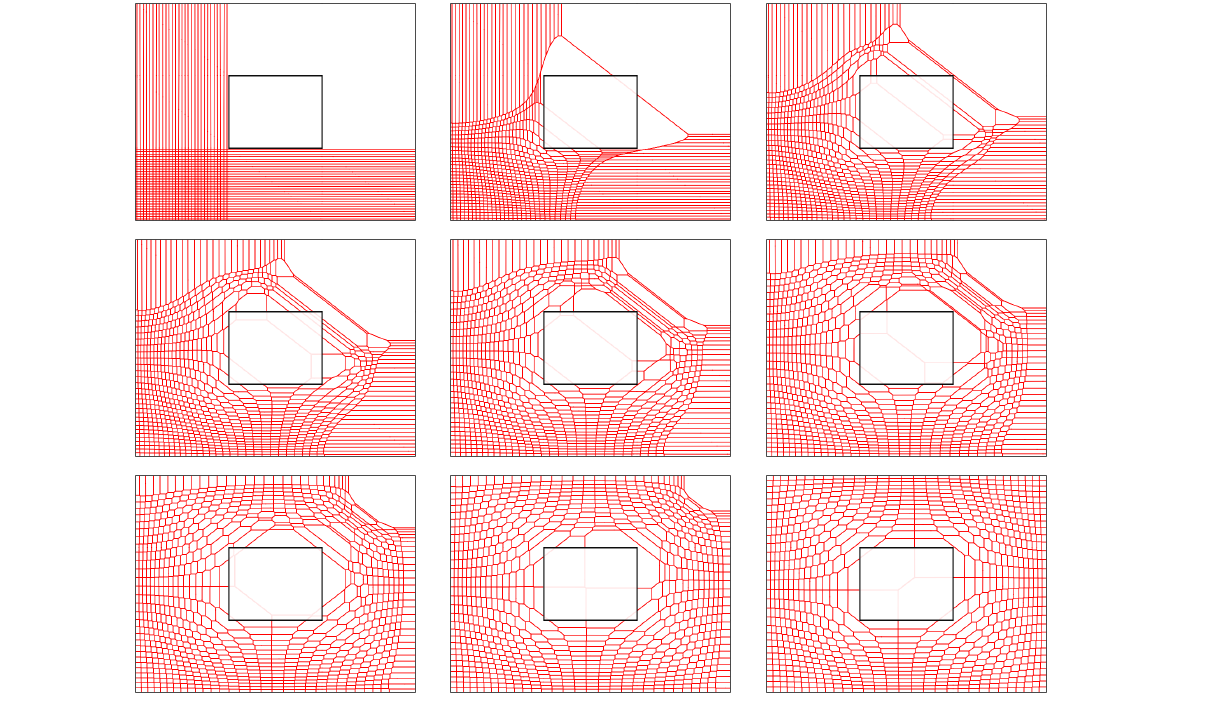
\includegraphics[width=0.8\linewidth]{Semi-discrete.png}}
          \caption{Numerical experiment}
        \end{figure}
\end{frame}


\begin{frame}{Semidual formulation: Wavelet estimator\footnotemark}
	Use M-estimator in truncated wavelet space to estimate the mapping $f$:
	\begin{itemize}
		\item Minimax rate
		\item Local Rademacher complexity
	\end{itemize}

	\par
	Problem: calculating the convex conjugate is very difficult, especially at high dimension.
	\footnotetext{Jan-Christian Hutter and Philippe Rigollet. Minimax rates of estimation for smooth
optimal transport maps. arXiv preprint arXiv:1905.05828, 2019.}
\end{frame}


\begin{frame}{Semidual formulation: GAN\footnotemark}
	Instead of calculating convex conjugate, one can directly use NN to parametrize function $f, f^*$, i.e. solve
	\bequn
		\inf_{f \in ICNN, g \in ICNN} \mbE\lb f(\nabla g(Y)) - f(X) + \la Y, \nabla g(Y) \ra \rb.
	\eequn
	\begin{figure}[H]
          \centering
          \centerline{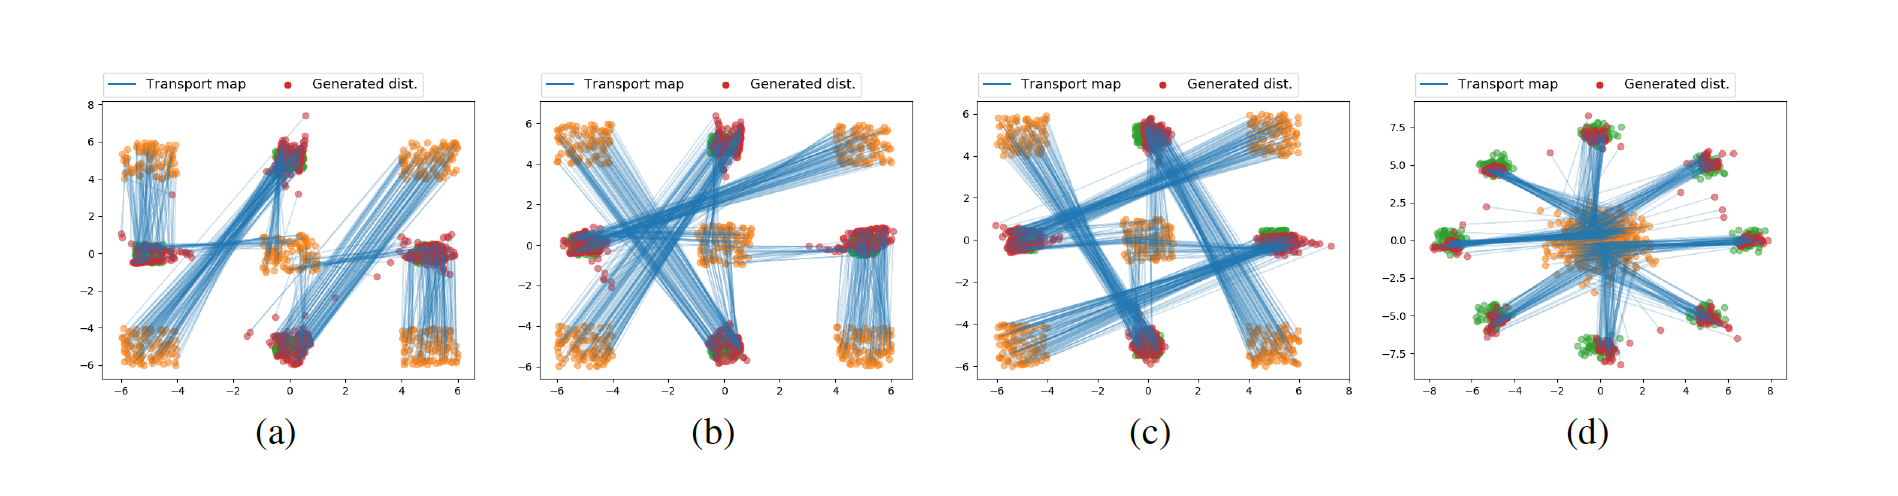
\includegraphics[width=1.2\linewidth]{GAN.png}}
          \caption{Numerical experiment}
        \end{figure}
        \footnotetext{A. Makkuva et. al, Optimal transport mapping via input convex neural networks, 2019}
\end{frame}


\begin{frame}{OT in the Spiked Transport Model}
	Spiked model:
	\bequn
		\begin{aligned}
			\mu^{(1)} & := Law(X^{(1)} + Z),		\\
			\mu^{(2)} & := Law(X^{(2)} + Z)
		\end{aligned}
	\eequn
	$X^{(1)}, X^{(2)}$ support on $U \in \mbR^d$ with intrinsic dimension $k \ll d$. Common part $Z$ supports on $U^{\perp}$.
	\par
	WPP (Wasserstein projection pursuit) estimator:
	\bequn
		\begin{aligned}
		\wtd W_{p,k}(\mu, \nu) & = \max_{U \in V_k(\mbR^d)} W_p(\mu_U, \nu_U),		\\
		\wht W_{p,k} & = \wtd W_{p,k}(\mu_n, \nu_n).
		\end{aligned}
	\eequn
	$\mu_U$ is 
	
\end{frame}


\begin{frame}{OT in the Spiked Transport Model}
	Good news: overcome CoD
	\begin{Thm}
		Let $(\mu^{(1)}, \mu^{(2)})$ satisfy the spiked transport model, for any $p \in [1, 2]$, if $(\mu^{(1)}, \mu^{(2)})$ satisfy the $T_p(\sigma^2)$ transport inequality, then the WPP estimator $\wht W_{p, k}$ satisfy
		\bequn
			\mbE \lv \wht W_{p, k} - W_p(\mu^{(1)}, \mu^{(2)}) \rv \leq c_k\lp r_{p,k}(n) + \sqrt{\frac{d\log n}{n}} \rp.
		\eequn
	\end{Thm}
	Bad news:
		There is not a polynomial time algorithm to calculate the WPP.
\end{frame}


\begin{frame}{Projected Wasserstein distance}
\end{frame}


\begin{frame}{Other interesting topics}
\begin{itemize}
	\item Multi-marginal OT and density functional theory (DFT)
	\item OT and GMM
\end{itemize}

\end{frame}




\end{document}